\chapter{Implementation}

	\section{Infrastructure}
		
		\subsection{Team management}
		
			Considering the kind of event bounded to the game usage, something gets clearly on mind: the team registration must be done long \emph{before} the event.
			
			For this, a simple website will be set-up. 
			Teams will be able to enrol for events, specifying the emails of all team members and a reference person which will take care of the team management (eg. player removal or substitution).
			In this way organizers will be able to directly communicate with all players of a given event.
		
		\subsection{Data storage and manipulation}
			
			Instead of relying on an old-style SQL database accessed from a PHP/Java environment, the data management is achieved using a new platform: Firebase.
			Firebase does a great job keeping data in sync between various devices and offer a powerful set of API, together with a strong system of data access rules.
			The only flaw is that queries on data are not so simple to perform and must be done using nested calls to the database.
		
		\subsection{Game}
		
			Being backed by Firebase I initially thought a backend server wasn't really needed, and i could implement some sort of all-in-app game logic.
			Unluckily, I soon realized that game phases, together with some game conditions checks, needed a centralized code to be performed.
			Actually this constraint is more a design-driven choice than a mandatory one: all the game logic \emph{could} be realized directly on the app, synchronizing between all devices, but this would result in messy code and open some security issues with which I would have needed to deal in the final stages of the project.
			Considering this, I decided to follow the KISS (Keep It Simple, Stupid) approach and separate the two aspects of the game.
			
			\subsubsection{Game logic}
			
				To support the game logic, a Java task on the server will run in loop interacting with real time database observing the actions being made by the players and eventually acting on his own to modify the game status.
				
				It takes care of:
				\begin{itemize}
					\item \textbf{initialization:} preparatory steps to execute before a match take place (initial status, board set-up);
					\item \textbf{phases:} manages phase changes and the timers associated with it;
					\item \textbf{objectives:} check every turn if a team reached his objective;
					\item \textbf{events:} manages the probability of an event to take place, its random choice between the available ones and applies his effects;
					\item \textbf{status reset:} every temporary status changes (zones power-ups and events effects) is reset to his original status at the end of turn;
					\item \textbf{power-up:} applies effects of the power-ups;
					\item \textbf{log:} record all match actions and operations in order to enable post-match studies and replays.  
				\end{itemize}
				
				The many timers that the game logic will need to share with the app will be saved on the database as their expiration date. In this way it's possible to every device in any moment to calculate the missing time to the expiration and set an internal time-out on their own.
			
			\subsubsection{Players logic}
			
				Player logic, instead, is managed by the app running on every device, which communicates directly with the real time database.
				
				It takes care of:
				\begin{itemize}
					\item \textbf{messenger:} a dedicated messenger will be provided to allow an in-game communication between team members;
					\item \textbf{localization:} keeps track of players last known position and last time he was active;
					\item \textbf{roles:} the role and action selection system will be entirely done by the app between the players, the server will only observe those operations;
					\item \textbf{board visibility:} which part of the board, which other players and which markers to show to each player will be decided by the app, depending on the role and location of current player.
				\end{itemize}
			
	\section{Work flow}
	\label{workflow:general}
		
		The game has a multiphase structure, one of which is turn based (the more important, the actual "gaming" part).
	
		\subsection{Inactive}
		
			The game has not yet been initialized, it's the default value when there is no game available.
	
		\subsection{Initialize}
		
			In this phase we set-up the game performing various ordered steps:
			
			\begin{enumerate}
				\item The board centre and radius are fetched from the database;
				\item Clean all data from previous game, in particular the random event probability and the turn counter are set to 0;
				\item Instantiate random events and reset set them as eligible to be drawn;
				\item Instantiate zones;
				\item Generate the board;
				\item Load zones info (centre coordinates, perimeter points, cost, description, etc.) and status (initially calm) into the database;
				\item Randomly chose the starting zones, setting them as chaotic;
				\item Retrieve teams and units from the database;
				\item For every team: 
				\begin{enumerate}					
					\item For every member of the team:
					\begin{enumerate}
						\item Select the starting zone with fewer units already assigned to it;
						\item Assign the unit to that starting zone;
						\item Set unit starting position to the centre of that zone, reset his last position and last beat values, set him as not ready to start the game;
						\item Increase the counter that keeps track of the users that play this game;
					\end{enumerate}
					\item Randomly chose an available objective and assign it to the team;
					\item Set the initial team's money reserve;
				\end{enumerate}
			\end{enumerate}
		
		\subsection{Prepare}
		
			During this phase, the units must reach their starting point: once everyone is within 10 meters from it, all listeners on the database are initialized and then the game is started.
		
		\subsection{Start}
		\label{workflow:start}
			
			This is the core phase of the game: it's a loop which every turn execute three logical sub-phases.
				
			\subsubsection{Control}
			
				Here the turn preparation is done: this part does not interact with the users in any way, considering that are mostly checks and various game status automatic changes.
			
				The first check performed is on the victory criteria: all teams' objective is checked against the current game status. If one of them is fulfilled, the games ends.
				
				Then, as first operation of the new turn, the turn counter is increased, its value is updated on the database and all temporary conditions are reset to their defaults.
				
				The second check is on the random event: if there is at least one available event to fire out, a randomly generated percentage number is tested against the current event probability and, if it's lesser or equal, the event is fired and the event probability is reset to a minimum value.
				In case the probability is set to 0.00 (possible only if it's the first turn), it is instead set to a minimum value and the test is skipped.
				
				Lastly, the bonus gained by the controlled zones is applied.
				
			\subsubsection{Roles}
			
				Here the roles selection system is activated and players will choose their role for that turn following the rules explained in \autoref{nolead:role}.
				The server will manage the timer of four minutes.
				
			\subsubsection{Actions}
				
				After giving the role, another timer, one minute long, is set to let them choose the action.
				
			\subsubsection{Money}
				
				Lastly, the money are taken by the players from team reserve as explained in \autoref{nolead:money}.
				This sub-phase also last one minute.
							
			\subsubsection{Turn}
			
				Here the real game take place: the server will keep a timer of fifteen minutes during which the players can act following their team objectives or disrupting others plans.
				Every action will be performed directly on the app communicating to the database without server interaction, but this does not mean that it will stay idle: every action made on the database, as well as every player movement, will be recorded by the server on a log file from which will then be possible to re-run the match replay in order to get statistics and to study it.
			
		\subsection{End}
		
			All players are notified that the game is ended and who's the winner, then a gathering point is given to all players that must reach it in order to meet-up with organizers and continue the event: likely the winner team will be awarded at this point with the possible prize.
			
	\section{Data model}	
		
		Data are modelled both on Firebase with his internal rules and in Android/Java with classic Java interfaces/classes.
		Android model is a simplified version of the Java one, with many fields which are changed from custom classes to simple strings, because the clients only need a subset of the operations needed by the server and cannot access all informations (many are restricted based on who's reading them).
		
		\subsection{Firebase model}
			
			In Firebase there is no concept of "data model" and the data structure definition de facto relies on the powerful yet flexible rule system which manage data access and manipulation.
			The rule system allows to validate incoming data with a JavaScript-like language encapsulated in a JSON and to define constraints, for examples, on which children a particular branch must have in order to be valid. This can be seen as defining a constructor in Java which enforce the initialization of mandatory fields.
			
			Considering that some lines are pretty much the same over various rule definitions, some kind of legend can be useful to cover the more common ones.
			
			\begin{itemize}
				\item \lstinline|".write" : false| \\ when no \lstinline|.write| rule is defined, it's is assumed to be this one for that level, because \lstinline|.write| rule default to \lstinline|false| when not specified;
				\item \lstinline|".validate" : "newData.hasChildren(['field1', 'field2', ...])"]| \\ if this branch is defined, then the specified fields must be present defined as well;
				\item \lstinline|"$var" : { ... }| \\ a wild-card which goes one level deeper in the branch, while keeping a reference to the key in which we are in, which can be used as a variable inside that scope rules. For example, in a branch \lstinline|dinosaur| with a collection of dinosaurs by name, the \lstinline|$dino| will contain the name of the dinosaur in which branch we are in;
				\item \lstinline|{ ..., ..., "$other" : { ".validate" : false } }| \\ any field different from the ones specified cannot be defined.
			\end{itemize}
			
			Firebase model is obviously simpler and looser than it's Java counterpart and has at top level only four branches.
			
			
			\subsubsection{Game}
			
				\lstinputlisting[caption=Game branch rules,
								firstline=3,
								lastline=63]{main/listings/firebase.json}
				
				All data needed to manage a game instance is contained here.
				Everybody can read at this location, but no one (except the server service account) has write permission, as shown by line~\ref{firebase:game:read} and the absence of the \lstinline|.write|.
				
				\paragraph{status - line~\ref{firebase:game:status}}
				Represent the status in which the game can be, as seen in \autoref{workflow:general}, plus \emph{PAUSE} and \emph{RESUME}.
				His Java counterpart is an enumeration class, and his content \emph{must} reflect the literal representation of that enumeration.
				This is used by the application and the server to check in which status the game is, considering that both are designed to take into account crashes and disconnection and just resume where the game was left as soon as they reconnect.
				Some application components, like the one which display the users on the map as described in \autoref{focus:map}, even use this information to alter their internal status and change their appearance.
				
				\paragraph{phase - line~\ref{firebase:game:phase}}
				Works in the same way, and with similar use cases, to the status field.
				Keeps track of the current phase while in \emph{START}, as seen in \autoref{workflow:start}.
				
				\paragraph{board - line~\ref{firebase:game:board}}
				Used mostly during \emph{INITIALIZE} operations to generate the game board, see \autoref{focus:board}.
				Contains the centre and radius of the board itself.
				
				\paragraph{unitsToWait - line~\ref{firebase:game:wait}}
				Used during \emph{PREPARE} to keep track of how many units have yet to reach their starting position.
				It's initialized with the total number of players during \emph{INITIALIZE} and decremented by 1 every time a unit reach his starting position.
				Instead, if a unit who already reached it move away from it, the counter is increased by 1.
				When it reaches 0, the server updates game status to \emph{START} and all client (who previously set a listener on it), will move from prepare activity to game activity.
				
				\paragraph{timer - line~\ref{firebase:game:timer}}
				Used during \emph{START}, is the moment in which the currently active timer will expire. It's updated by the server service account each time a timer expires and a new one is set and read by all client devices to synchronize with the game workflow.
				
				\paragraph{turn - line~\ref{firebase:game:turn}}
				Used during \emph{START}, is the turn counter. Considering the game structure, which can potentially go on forever until a team wins, this could seem useless, but to avoid exactly this scenario one objective has been designed to cut the game after 7-8 turns.
				This countermeasure has been taken to address multiple constraints, mainly battery drain, game pressure and players concentration.
				
				\subparagraph{battery drain}
				Mobile games always find a fierce opponent in battery drain, just by considering that the screen must always be on while playing.
				In this case, the problem is even more accentuated, given that the game requires not only the screen to be turned on, but also GPS, internet connection and, while in augmented reality mode, even the camera steadily capturing and processing images.
				A single turn is composed by 20 minutes, asking the battery to support all this consumption for a total of 140-160 minutes by his own is pretty unrealistic, unless all players got an high end smart-phone.
				Another way to address this problem could be to give each player a power bank and USB cable, which will be a fall-back in case 7 turns will prove themselves to be too short for other teams to compete.
				
				\subparagraph{game pressure}
				Most games are played to relieve stress. This is not the case. In fact, this game can be considered like a competitive game and the pressure over players must stay high during all the match. Removing the turn limit could lead some people to relax and not taking the game seriously, ruining the game both for their opponents and team-mates.
				Unlimited play time also let the user correct their mistakes, because a strategy defect in a turn can be fixed during the following 3-4 turns while keeping on with the team objective: this again make the game longer and does not punish enough who made a mistake, leading to a game where taking a risk has low to zero consequences.
				There will be plenty of time to relax before and after the game, but \emph{during} the game, pressure must stay high.
				
				\subparagraph{players concentration}
				As a student and worker, I know that human concentration has limits. The game structure based on 5 minutes of decision making followed by 15 of running around and doing stuff has been thought taking this into consideration, but it's impossible to stay steadily concentrated on something for more than two hours.
				To ensure players fun, the game must be as short as possible, or they will quickly get bored.
				
				
				\paragraph{event - line~\ref{firebase:game:event}}
				Used during \emph{START}, keeps track of the random events probability and of which didn't happened yet (every event may take place only one time). This info could be, and actually is, stored directly in the server, but it's copied and kept up-to-date also on Firebase in order to prevent data loss upon server crash. Moreover, putting it here, we can let the players know which events can still happen.
			
			\subsubsection{Team}
			
				\lstinputlisting[caption=Team branch rules,
								firstline=65,
								lastline=129]{main/listings/firebase.json}
				
				Information about teams are stored here.
				Everybody can read at this location, but no one (except the server service account) has write permission, as shown by line~\ref{firebase:team:read} and the absence of the \lstinline|.write|.
				The \lstinline|.read| command had to be moved out of the single team scope, otherwise units would be able to read every single team branch, but not the whole list. 
			
			
				\paragraph{color - line~\ref{firebase:team:color}}
				The color associated with this team. Considering that a visual representation is needed in order to display differentiate units on the board (both in the map and in the AR part), a random color chosen between the predefined ones is assigned to every team during the team registration. This color will be used every time there will be the necessity to show that an unit is of a particular team or to show the team generic information.
				It's stored like a color name, instead of an hex code, in order to directly use the \lstinline|Color.valueOf(name)| method present on Android (otherwise we would have to use the \lstinline|ResourceCompat| support class to get it and would have been resulted in less human-readable code); this could be changed if a more specific color selection is needed.
			
				\paragraph{name - line~\ref{firebase:team:name}}
				Specified during the team registration, it will be displayed to identify the team when required.
				
				\paragraph{objective - line~\ref{firebase:team:objective}}
				Randomly assigned during the game initialization, describes the victory criteria of the team.
			
				\paragraph{members - line~\ref{firebase:team:members}}
				All members of the team are listed within this branch, with the units key as the sub-branch key and \lstinline|true| value. This is an easy way to access the information from validation rules of other fields: checking if the branch \lstinline|team/<team_id>/members/<unit_id>| exists is the easier way to know if an unit is a member of a particular team.
			
				\paragraph{money - line~\ref{firebase:team:money}}
				Money reserve of the team. Both \lstinline|loan| and \lstinline|maximum| fields must always be set. At the start of the game \lstinline|loan| is initialized to 0 and \lstinline|maximum| to 10 coins.
				The money management works as explained in \autoref{nolead:money}.
				
				\lstinline|maximum| decreases accordingly to the loan given in \emph{MONEY} phase, so players from other teams can check how much coins have been given to units comparing the reserve before and after that phase, and increases again during the \emph{CONTROL} phase in which money from every unit gets back to the team reserve.
				When assassins demolish building of this team, half the price paid to construct it is refunded and therefore added to this field.
				
				\lstinline|loan|, instead, keeps track of the loan requested during \emph{MONEY} phase and must be comprised between 0 and the maximum money in the reserve. This is one of the few fields which are modifiable by units inside the team branch, but can be touched only by team members.
				
				\paragraph{roles - line~\ref{firebase:team:roles}}
				Role pool data. Both \lstinline|current| and \lstinline|maximum| fields must always be set. At the start of the game both \lstinline|maximum| and \lstinline|current| fields are set to the initial role poo: 2 cops, 2 assassins, 2 builders, 999 collectors, 0 untouchable and 0 multitasking.
				The role management works as explained in \autoref{nolead:role}.
				
				\lstinline|maximum| field is updated at the end of \emph{CONTROL} phase of every turn, after taking into account possible random events and zones power-up.
				
				At the very beginning of the \emph{ROLE} phase, \lstinline|current| child values are reset to be equal to the \lstinline|maximum| ones, then they're updated every time a unit choose his role or change his already chosen role. In this way, other units can easily see which roles are still available for them to choose.
				Those values cannot ever be negative and can be at least as much as their counterparts in \lstinline|maximum| field.
				This is one of the few fields which are modifiable by units inside the team branch, but can be touched only by team members.
			
			\subsubsection{Unit}
			
				\lstinputlisting[caption=Unit branch rules,
								firstline=131,
								lastline=192]{main/listings/firebase.json}
			
				Information about units are stored here.
				Everybody can read at this location, but only the unit itself (and the server service account) has write permission, as shown by line~\ref{firebase:unit:read} and~\ref{firebase:unit:write}.
				The \lstinline|.read| command had to be moved out of the single unit scope, otherwise other units would be able to read every single unit branch, but not the whole list.
			
				\paragraph{username - line~\ref{firebase:unit:username}}
				Unit username, as inserted during the registration. It's used to identify the unit in many different scenarios: on the map fragment, in AR activity, in the team management fragment, etc. Not to be confused with the email, needed for the login and saved together with the password in the Firebase Auth system.
			
				\paragraph{team - line~\ref{firebase:unit:team}}
				Team identifier of which this unit is member. It's a redundancy, we could check every team if this user is present in the \lstinline|members|) field, but in Firebase this is normal, considering the difficulty and limitation in query system.
				It's validated to be sure that the inserted identifier actually reference an existing team.
			
				\paragraph{lastOnline - line~\ref{firebase:unit:online}}
				If the unit is not currently on-line (see \autoref{model:presence}), this value represent the last moment in which he was seen on-line. This is used mostly by the game logger (\autoref{focus:log}) or to display how much time passed since a unit accessed the application. It's updated when the unit disconnect from the system, as explained in \autoref{focus:presence}.
				
				\paragraph{lastPosition - line~\ref{firebase:unit:lastpos}}
				The last GPS position in which the unit was seen. AR parts of the project are based on this field (and it's updates from all units) to show where other units are.
			
				\paragraph{zone - line~\ref{firebase:unit:zone}}
				The last zone in which the unit was seen. It's updated when the unit move out of his previous zone for at least 10 meters. This field is the main component of the visibility rule system used on the map, as described in \autoref{focus:map:visibility}. Can assume value from 0 to 9, where 0 means that the unit is currently out of the board, while values from 1 to 9 represent the zones with that number as key.
				
				\paragraph{startPosition - line~\ref{firebase:unit:startpos}}
				Used in \emph{PREPARE}, is the GPS position of the starting point of the unit. It's set in \emph{INITIALIZE} where units are equally distributed on 3 randomly chosen starting zones, and correspond to the zone centroid.
				When the user reach his starting point, it's asked to stay near it until all other units has reached theirs. They can move as far as 20 meters from it, if they go further, the application will notice and ask them to return to the starting point.
				
				\paragraph{ready - line~\ref{firebase:unit:ready}}
				Used in \emph{PREPARE}, record if the unit reached or not the starting point. Based on this, field we are able to distinguish from a unit which arrived to the starting point and then moved slightly away and someone which arrived near the starting point but never reached it for real, still resulting not ready to start the game. Every time a new unit set this field value to \lstinline|true|, he will also decrease by one the \lstinline|unitsToWait| field on the game branch.
				If the unit moves too far away from the starting point, the value is reset to \lstinline|false| and \lstinline|unitsToWait| will be increased by 1. 
				
				\paragraph{role - line~\ref{firebase:unit:role}}
				Used in \emph{START}, represent the current role of this unit. By default it's set as \emph{UNSPECIFIED}, value to which is reset at every \emph{CONTROL} phase.
				During \emph{ROLE} phase, may change several time while team members decide who'll take which role, then it cannot be modified until next \emph{ROLE} phase.
				The chosen role also impact on the actions which can be selected by this unit in the subsequent phase, \emph{ACTION} one.
				This field is one cornerstone of the game, because greatly influence visibility rules and interactions between units.
				
				\paragraph{action - line~\ref{firebase:unit:action}}
				Used in \emph{START}, stores the chosen action. It's updated in \emph{ACTION} phase and, while not influencing the visibility rules like the \lstinline|role| field, defines at a more fine level the interaction with other units. Usually every role grant access to the choice between 2 actions, except from the \emph{COLLECTOR} role which grant just one action. Using the \emph{MULTITASKING} power-up it's possible to select both the actions provided with every role, but this features has not been modelled yet, even if it will probably lead to changing the \emph{action} field from a \emph{String} to a \emph{List}.
				
				\paragraph{money - line~\ref{firebase:unit:money}}
				Used in \emph{START}, this field is used, in different phases, to record either the coins the unit ask to borrow from team reserve or the coins he's carrying with him.
				
				It's possible to get money in 3 ways:
				\begin{description}
					\item[asking a loan] as described in \autoref{nolead:money}, in \emph{MONEY} phase;
					\item[collecting coins] if the \emph{COLLECTOR} role has been chosen, using AR to find and pick up coins, in \emph{TURN} phase;
					\item[robbing other units] if the \emph{ASSASSIN} role has been chosen, assassinating someone which was carrying coins, in \emph{TURN} phase.
				\end{description}
			
				Money can be used by builders to construct a building, paying a cost which differs from zone to zone, depending on the power-up usefulness.
			
			\subsubsection{Zone}
			
				\lstinputlisting[caption=Zone branch rules,
								firstline=194,
								lastline=277]{main/listings/firebase.json}
								
				Information about board zones are stored here.
				Everybody can read at this location, but no one (except from the server service account) has write permission, as shown by line~\ref{firebase:zone:read} and the absence of the \lstinline|.write|.
				The \lstinline|.read| command had to be moved out of the single zone scope, otherwise other units would be able to read every single zone branch, but not the whole list.
				It must be noted that zone identifier must be an integer between 0 and 9, in order to make the \lstinline|near| field work correctly.
				
				\paragraph{description - line~\ref{firebase:zone:description}}
				Zone description, which is usually related to the power-up effect.
				
				\paragraph{cost - line~\ref{firebase:zone:cost}}
				Coins which must be paid to construct a building on this zone. To be able to do so, builders must carry with them at least this amount of coins. Upon a building demolition, half the cost is refunded to the owner team. Upon constructing a building, instead, the team gain the zone power-up, taking it from the previous possessor, if any.
				
				\paragraph{center - line~\ref{firebase:zone:center}}
				GPS position of the centre of this zone. It's used in \emph{PREPARE} as starting point for units.
				
				\paragraph{perimeter - line~\ref{firebase:zone:perimeter}}
				Collection of GPS position of all vertex composing the zone perimeter. It's set for the first and only time in \emph{INITIALIZE} and used to print the game board on the map and to check if a unit is in this zone or not. It's important to note that vertexes must be ordered, otherwise the perimeter would result in no more than a scribble on the map.
				
				\paragraph{near - line~\ref{firebase:zone:near}}
				Collection of zones near to this one, needed to execute some power-up effects.
				The added values are checked to be actually reference to other zones.
				
				\paragraph{chaotic - line~\ref{firebase:zone:chaotic}}
				The status of this zone: \lstinline|true| if chaotic, \lstinline|false| if calm. Builders cannot construct in a chaotic zone, while assassins cannot assassinate units in a calm zone. This field can be updated only by the units which chose \emph{CALM} or \emph{PANIC} actions in this turn.
				
				\paragraph{controller - line~\ref{firebase:zone:controller}}
				Team which holds control on this zone. The control mechanic is needed for an objective, which requires to gain control of 4 zones to win the game. A team is called "controller" of a zone if the sum of his buildings and units in that zone is higher than the one of every other team in game. This mechanic is better explained in \autoref{focus:control}.
				
				\paragraph{units - line~\ref{firebase:zone:units}}
				List of units currently in this zone, it's used to check which teams control this zone and only the unit itself can add/remove his child branch at this path. Of course, the it must be a valid and authenticated unit.
				
				\paragraph{buildings - line~\ref{firebase:zone:buildings}}
				List of buildings constructed in this zone. Every building must have a \lstinline|owner| field which stores his owner team id. Only units which chose \emph{BUILD} or \emph{DEMOLISH} action for this turn can update data at this location (constructing or demolishing a building).
			
			\subsubsection{Presence}\label{model:presence}
		
				\lstinputlisting[caption=Presence branch rules,
								firstline=279,
								lastline=291]{main/listings/firebase.json}
									
				This branch support the presence management system, which will be discussed in more detail in \autoref{focus:presence}.
				Everybody can read at this location, every unit can write here as well, but only in the sub-branch based on their id, as shown by line~\ref{firebase:presence:read} and~\ref{firebase:presence:write}.
				The \lstinline|.read| command had to be moved out of the single unit scope, otherwise other units would be able to read every single unit branch, but not the whole list.
				The only value which every unit branch can assume is \lstinline|true|, which states that unit is currently on-line. Conversely, if the branch with the given unit id does not exists, the unit is off-line.
			
		\subsection{Java/Android}
		
			\subsubsection{Game}
		
			\subsubsection{Team}
			
			\subsubsection{Unit}
			
			\subsubsection{Zone}
			
			\subsubsection{Board}
			
			\subsubsection{Building}
			
			\subsubsection{Objective}
			
			\subsubsection{Role}
			
			\subsubsection{Action}
			
	\section{App workflow}\label{app:workflow}
	
		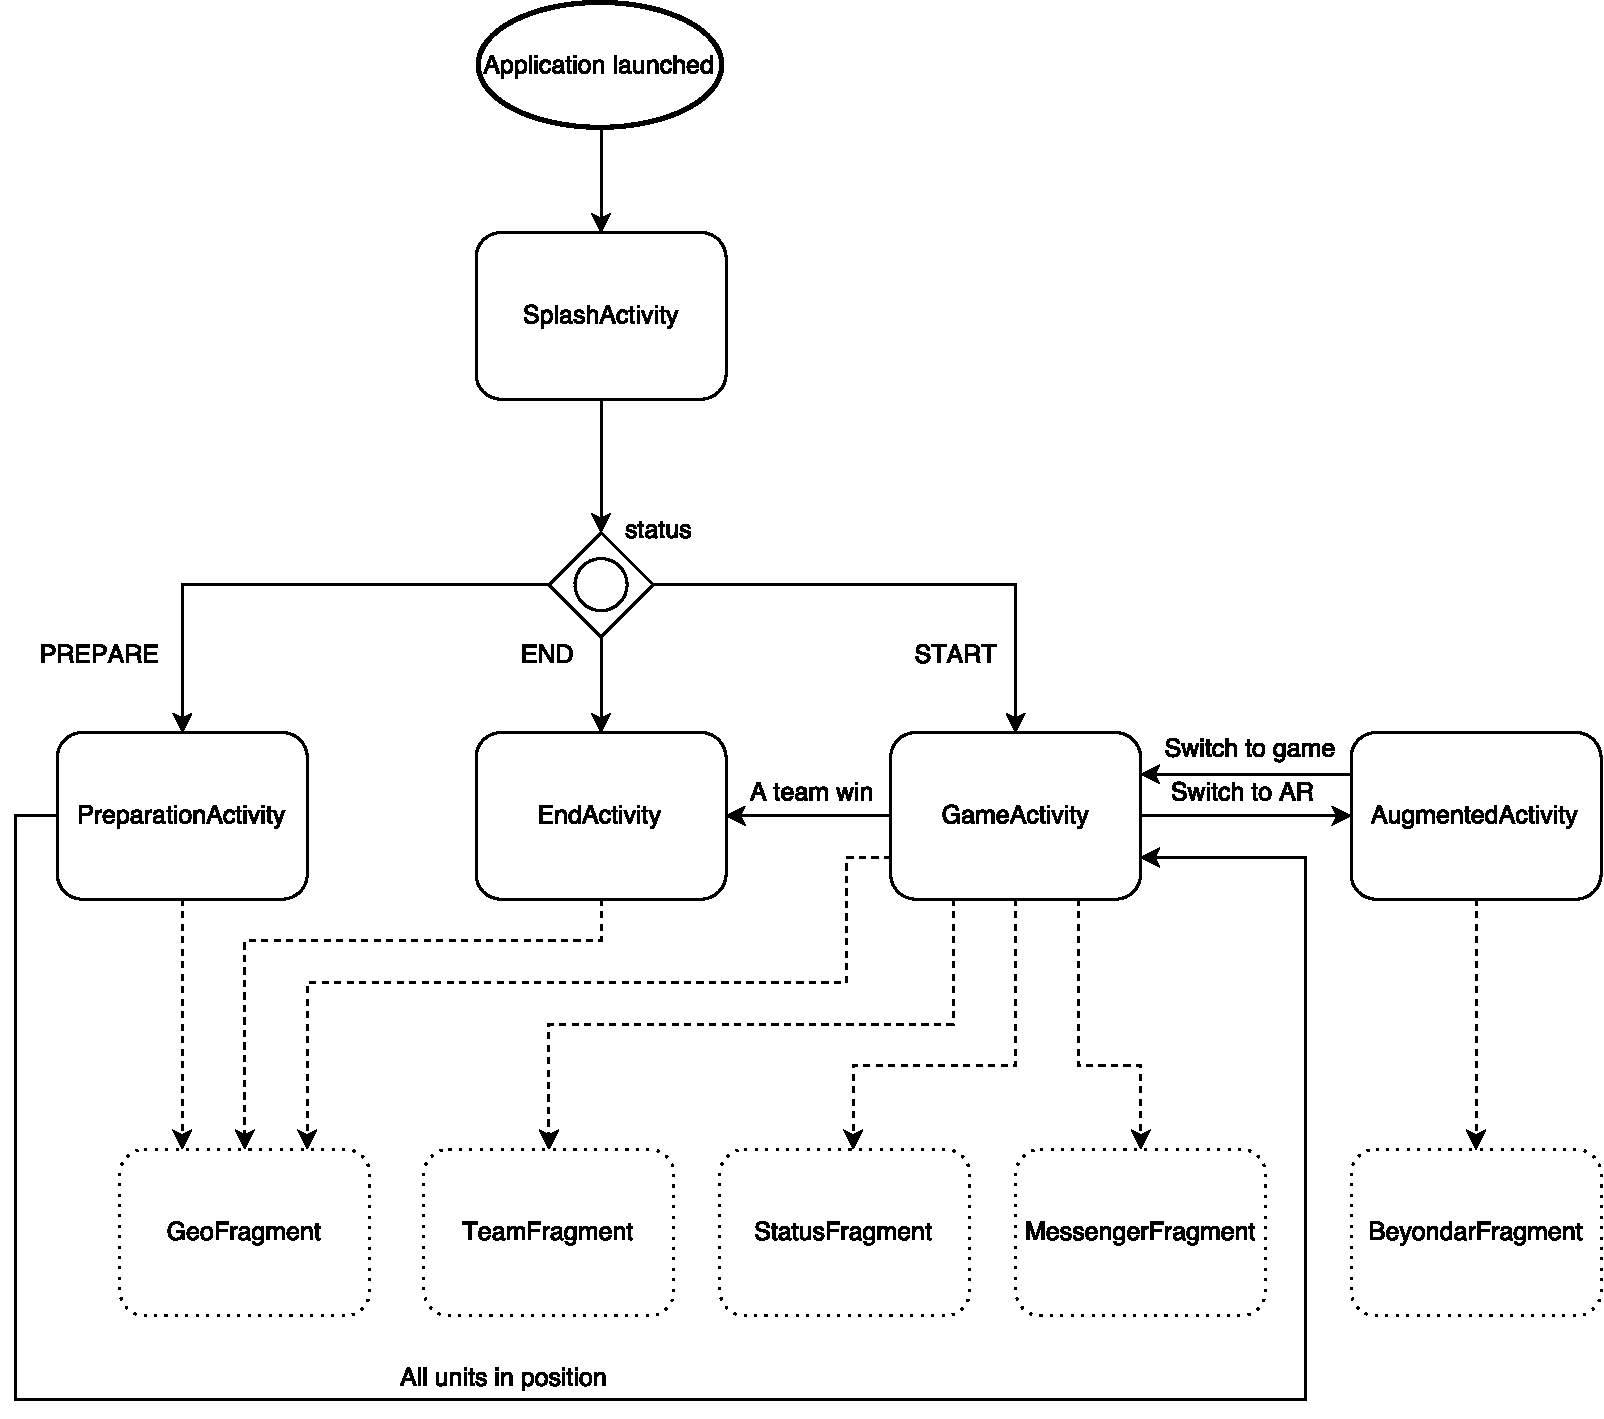
\includegraphics[width=\textwidth]{androidflowchart}
		
		Together with the game mechanics and rules description, a prototype of the game has been prepared for Android systems and works from API 16 onward.
			
		Due to limited time and external job constraints, I wasn't able to finish the prototype, which is currently incomplete in some of his modules: messenger system has not been implemented, the augmented reality part which used the camera (which had been prepared as the first module) has not been properly connected to the prototype and with the action system, status fragment which shows info about other teams has not be implemented, the end game activity has not been implemented (even if it's more or less a copy of the preparation one).
			
		Following, a description of the features of every activity and fragment which composes the application.
		
		\paragraph{SplashActivity}
		
		It's composed by two alternatively layouts, one for login and the other for the loading part.
		Its main purpose is to perform the user login and pre-load all useful informations for the subsequent activity, which will then start after understanding which status the game has in that moment.
		Everything it does is described in more details in \autoref{focus:splash}.
		
		\paragraph{PreparationActivity}
		
		It's composed solely by an instance of the GeoFragment and its main purpose is to guide players to their starting point, forcing them to wait there when they reached it. When everybody is in the right place, it start the following activity: \lstinline|GameActivity|.
		
		\paragraph{GameActivity}
			
		It's composed solely by a view pager (a group of tabs) which manages various aspects of the game.
		When a team successfully accomplish his objective, it starts the last activity of the game: \lstinline|EndActivity|.
		
			\subparagraph{GeoFragment}
			
			It's the more important fragment of the activity, because it let you see the board, where other units are and many informations about the AR layer of the game.
			At code level, it's a wrapper around a \lstinline|MapFragment| (from Google Maps Android library) which takes care of managing the board with the zones of which it's composed, units position and the related visibility rules, AR objects which spawns around and many others tasks: its working flow is described later in \autoref{focus:map}.
			
			\subparagraph{TeamFragment}
			
			It's composed by four parts, each visible only during certain phases except the forth one:
			\begin{description}
				\item[role management] displays the roles available during the \emph{ROLE} phase and let the unit to select its own;
				\item[action management] displays the actions available, related to the chosen role, during the \emph{ACTION} phase and let the unit to select its own;
				\item[money management] shows how many money are present in the team reserve and let unit borrow some of them in the \emph{MONEY} phase;
				\item[teammates status] a list showing the role, action and borrowed money of every other unit in the team, it's visible in all phases of the game.
			\end{description}
			
			With this components, it manages three out of four phases of which the game is composed.
			
			\subparagraph{StatusFragment}
			
			It's composed by a general status bar, which show some general info about the game (current turn, how many and which random events are left, etc), and a list of team summary cards, one for each team playing (number of controlled zones, total money in their reserve, etc.).
			
			\subparagraph{MessengerFragment}
			
			It's similar to every other messenger system (Whatsapp, Allo, Facebook Messenger) and is implemented using the Firebase Cloud Messaging, not needing all the more advanced features (eg. photos and videos).
		
		\paragraph{AugmentedActivity}
		
		It's a \lstinline|FrameLayout| containing a \lstinline|BeyondarFragmentSupport|, a wrapper of a normal fragment enhanced to display the camera capture as background, and an AR overlay which displays things based on the position of various objects and units.
		It's work is to allow interaction between units and between units and AR objects, its behaviour is better described in \autoref{focus:augmented}.
		
		\paragraph{EndActivity}
	
		It's the last activity of the game, and it's composed solely by an instance of the GeoFragment as \lstinline|PreparationActivity|.
		Its main purpose is to gather players to the end position, where the winner will be awarded. When everybody has reached it, the game is finished and the application force a logout of all players, changing the game status to \emph{INACTIVE}.
	
	\section{Main technological issues}
		
		While working on the project, I had to decide how to address particular problems, which resulted in some complex piece of code.
		Hopefully, the explanation about how I managed to overcome them will be helpful for someone who'll need to follow this same path.
		
		\subsection{Board generation}\label{focus:board}
		
			During the process of rules adaptation from the reference board-game to the app, the definition on how the board should have been as seen in \autoref{design:board}, occupied some time.
			
			The initial idea was to obtain a randomly generated, asymmetric board contained in an irregular polygon defined by the event organizers.
			In this way, the playing ground could have been set to fit into different real-world city-related shapes (in Reggio Emilia case, the irregular hexagon made by the beltway was the most obvious shape to use).
			In addition, a randomly generated board would have prevented teams to study strategies based on the already known map and would have forced them to improvise a new strategy while studying the map in \emph{PREPARE}.
			
			Unluckily, this kind of board generation almost immediately looked too advanced to be realized in the short time available, so I settled to a more simple regular shape formed starting by a given centre and a radius.
			
			The more simple and regular polygon that could be used was of course a circle, and that was my choice until I had to deal with Google Maps management of polygons. Circular shape was perfect for the board perimeter by himself, but I also needed the zones perimeter for in-game mechanics (check in which zone each unit is, manage zone crossing, random point generator inside a given zone, etc) and this was impossible to archive using the build-in circular shape of Maps API.
			The second thought was to replicate the external circular shape with polygons with a lot of points, but that would have leaded to possible performance issues.
			In the end, as seen in the board image in \autoref{design:board}, I decided to stick to a particular shape where the central zone is composed by 8 sides (one vertex every 45 degrees), four more zones are contained between the first zone perimeter and a ring composed by 16 sides (one vertex every 22.5 degrees) and last 4 zones are contained between the first ring and a second ring composed by 24 sides (one every 15 degrees).
			Zones between the second ring and the first one are shifted by 45 degrees because we wanted every zone to touch at least other 4.
			
			The fastest way to obtain all zones vertex, possibly also the simplest way apart from hard-coding the GPS positions of all zones, was to directly calculate the perimeter of every ring (the two mentioned earlier plus the central zone perimeter), putting all vertex in a multidimensional and ordered array representing zones perimeters.
			This is possible thanks to the fact that zones are all adjacent, which means that many vertex are in common with multiple zones, it's only necessary to put them in the right order.
			
			At code level, this is achieved with three \lstinline|for| loops pretty similar one to the other, which lead me to think that it could be optimized even further by using polar coordinates, but the code is already complex as it is and for now the result is acceptable.
			The first and last loops calculate vertexes clockwise, but the middle loop must do it anti-clockwise; this is done because having alternately spinning loops makes much simpler to save vertex of all zones already ordered and get a closed shape for the polygons, as seen in \autoref{board:alternate}.
			
			\begin{figure}[htp]
				\centering
				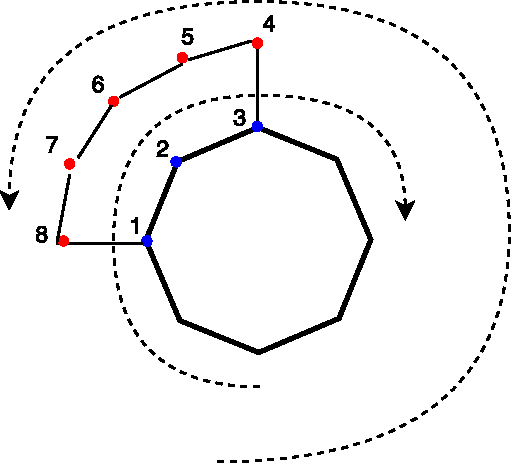
\includegraphics[width=.5\textwidth]{boardrounds}
				\caption{Graphical representation of alternate vertex calculation, showing the perimeter of one of the zones of the first ring}\label{board:alternate}
			\end{figure}
			
			Inside this loops, all points are obtained by starting from the board centre and calculating the new point based on the radius of the given ring and the offset angle which change at every iteration.
			
			\lstinputlisting[caption={Utility method, get new GPS position from given point, distance (ring radius) and angle}, firstline=158, lastline=171]{main/listings/boardfactory.java}
			
			It has to be noted that the board perimeter is not saved anywhere: only zones polygon are stored and printed upon the Google Map, for various reasons.
			First of all, we must be able to click on zones polygons on the map for some in-game mechanics (getting zone info like which teams owns his power-up or how many other units are present in the zone), so we have to save them anyway.
			Secondarily, the only reason for which we need the board perimeter is to check if someone exits it, but we can achieve the same information by checking if a position is inside any of the zones we saved: if it's not, the unit exited the board.
			
			\begin{figure}[htp]
				\centering
				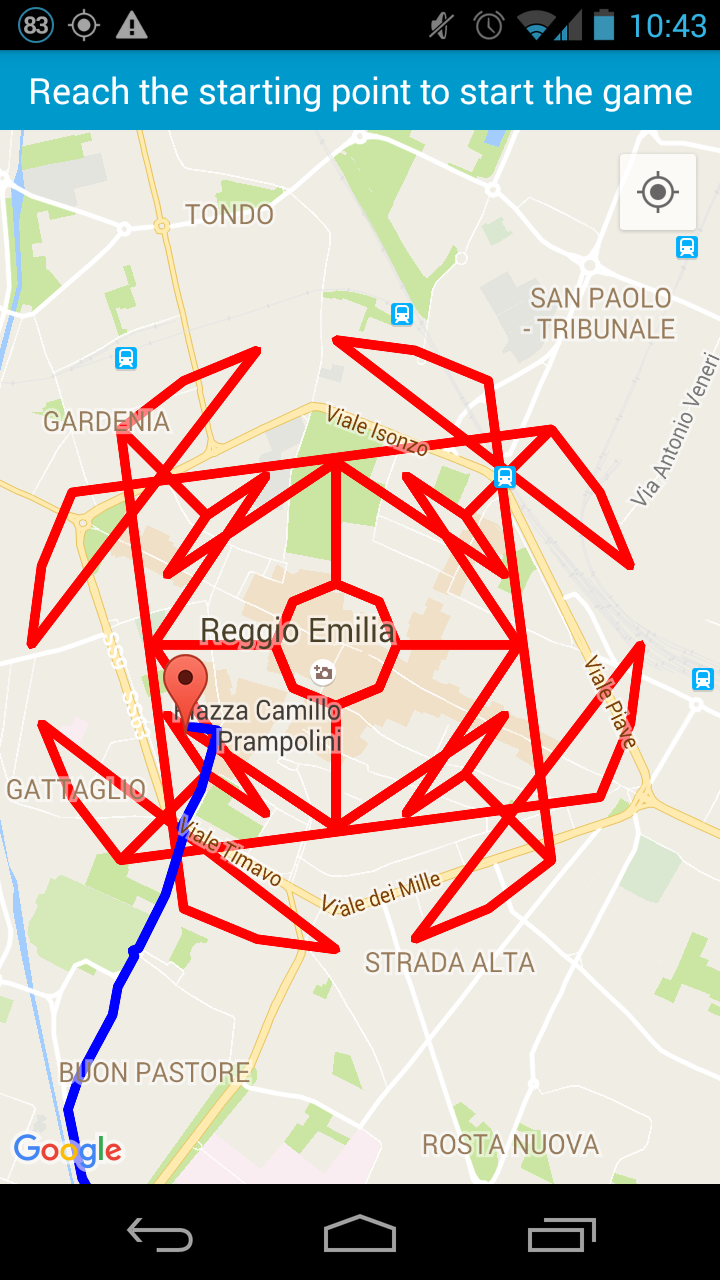
\includegraphics[width=.3\textwidth]{wrongboard1}
				\hfill % Stretches the space between images to align them to borders
				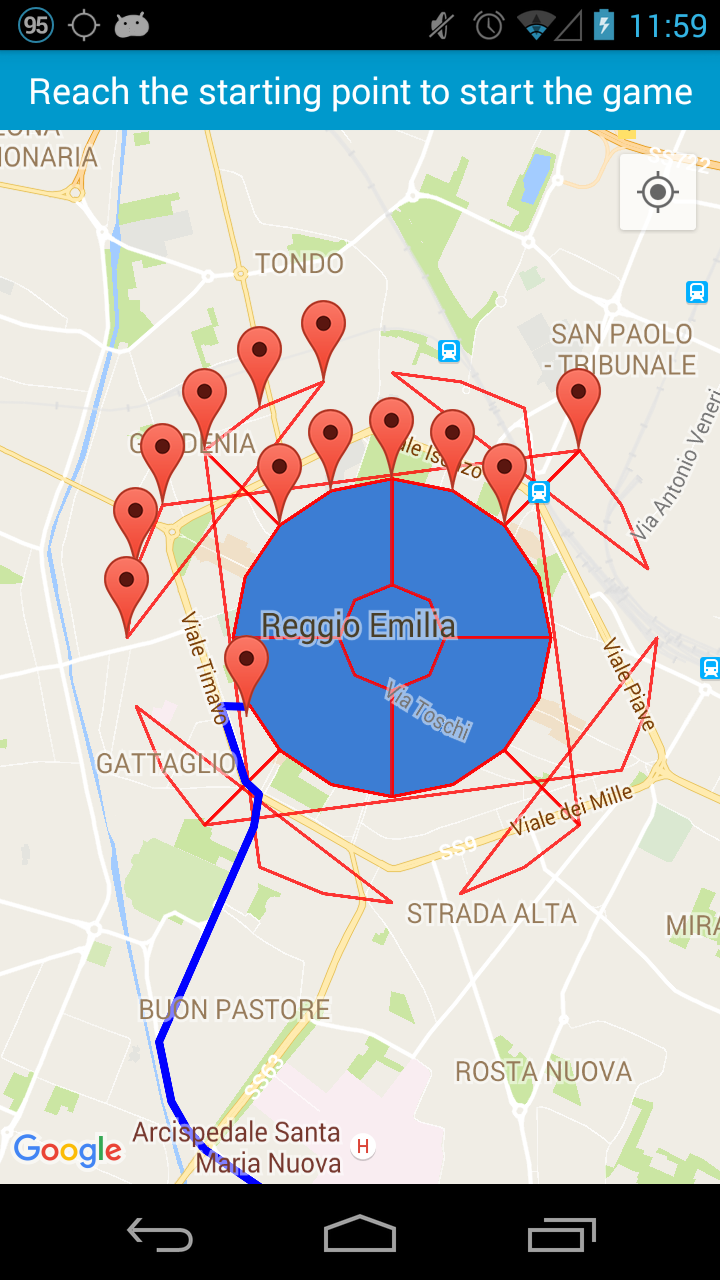
\includegraphics[width=.3\textwidth]{wrongboard2}
				\hfill
				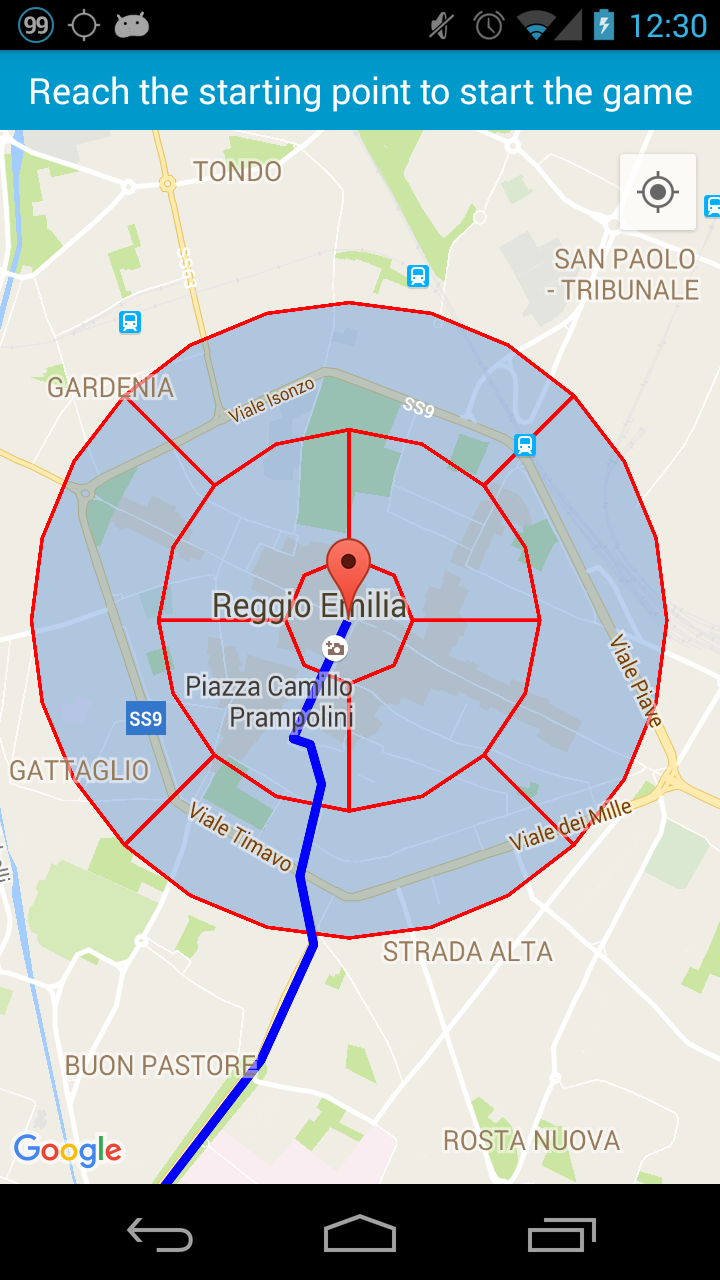
\includegraphics[width=.3\textwidth]{wrongboard3}
				
				\caption{Three board drawings trials while developing \lstinline|BoardFactory|}\label{board:mess}
			\end{figure}
			
			After some trial and error (\autoref{board:mess}), I managed to obtain the right shape, but the radius I used to calculate the rings was obviously wrong.
			Considering I wanted the zone to have the same area, I asked a friend of mine to run an R script to find which radius every ring must have in order to achieve it. Obviously the R script assumed the rings as circles, not as the weird shapes they actually are.
			
			After loops finish their run, the multidimensional array is used to fill in the perimeter \lstinline|ArrayList| of every zone on the board.
			
			The last part of the board fabrication is to make all zones aware of their neighbours. Unluckily, I could not think of a way to achieve this other than hard-coding it, and for now the map is simple enough to allow for this.
			
		\subsection{Timer mechanism}\label{focus:timer}
		
			Synchronizing phases between server and clients is pretty easy with Firebase: taken that the server manages phase timers by his own without crashing and updates accordingly the phase field on game branch, the devices have just to set a listener on it in order to know in which phase the game is.
			The task between less trivial when you add the fact that all device must have a synchronized countdown of the current phase.
			
			The first idea is indeed to store, together with the current phase, also the timer duration.
			In this way, every device connected could just set an internal timer, nearly synchronized with the one on the server and the problem is solved.
			
			But let's go further: what if the devices must be able to connect/disconnect at will and still have the synchronized countdown feature?
			The must obvious idea will be to add another field, perhaps the moment in which the timer has started, together with his duration.
			
			To spare a field (which, in Firebase, usually means sparing an asynchronous listener and a lot of trouble), my solution was to store, instead of starting time and duration, directly the expiration moment of the timer.
			For this to work, the time on every device and on the server must be the same. This is usually automatically managed by the operating system which uses internet to synchronize himself to the right time and can be takes as assured on the server machine, but on players smart-phones I have no control on the actual internal time of the device, which open the gates to possible glitches and cheats.
			
			Luckily Firebase comes to assist us on this as well: listening to the particular path \lstinline|.info|, a number of miscellaneous and useful piece of data can be accessed, one of them being the time offset between the local device and the Firebase server local time.
			
			Listening to \lstinline|.info/serverTimeOffset| value change allow us to detect the current offset from the server, store it and add it to the countdown timer that display the remaining time at every timer field change or device connection.
			
			To prevent every possible exploit, every time the timer field is changed on Firebase by the server, the local timer on every device is cancelled (if it was not expired yet), his onFinish callback executed and the new timer is set up.
		
		\subsection{Match logging}\label{focus:log}
		
			In order to better study the game mechanics effectiveness, it's useful to be able to replay all matches, which can used also in detecting possible cheaters or problems.
			
			For this, I set up a logging system which keeps track of all units' actions, as well as their movements, and various in-game events.
			
			The \lstinline|GameLogger| class is a singleton which statically provides a logger which writes to a file in the "/log" path, appending the creation timestamp to the log file name to log multiple game sessions.
			
			All server model classes implements the FirebaseSync interface, which ask to override the \lstinline|sync()| method.
			In this method, called at the end of the constructor, all listeners to useful info from Firebase are set.
			In this way, all instances will auto-update themselves listening for changes on Firebase and while doing so, they'll also log all the meaningful actions and events which are taking place during the match.
			
			After the game is completed, the structured log file will be set as input of an ad-hoc decoder which can then show a timeline from it, reproducing the events like a video.
			
			This ad-hoc decoder has not been developed yet, but it shouldn't be hard to implement. 
		
		\subsection{Random picker}\label{focus:picker}
		
			\lstinputlisting[caption=Random picker class]
							{main/listings/randompicker.java}
			
			A small but useful function which is missing from Java \lstinline|List| interfaces is the possibility to extract a random object from a given list.
			This may seem not useful, but nearly each game may need some kind of random extraction and also in other contexts (eg. testing purposes) a small function like this can come handy.
			
			In this project I made large use of randomly assigned values, eg. objectives distribution to teams, and a lot of parts I had not time to finish will heavily relies on random generation and extraction.
			
			For this reasons I created a small utility class to extract random values from a given list, composed by two methods:
			\begin{description}
				\item[pick] take the random seed of this thread, then randomly pick an integer value between 0 and the list size -1 and return the list element associated to that value. 
				\item[extract] same as pick method, but remove the extracted object from the list.
			\end{description}
		
			The picker uses \lstinline|ThreadLocalRandom| class instead of the more known \lstinline|Random| because, relying on asynchronous callbacks and on multi-threading, the synchronized access overhead to the process-global class may decrease performance a little.
			Plus, it's the recommended class to use, as written in Java 8 docs.
						
		\subsection{Random point generation}\label{focus:point}
		
			\lstinputlisting[caption=Random point generator class]
							{main/listings/randompoint.java}
			
			To implement most of the AR interaction, it's needed a way to generate random points, usually inside a given perimeter (specifically, inside a zone).
			
			Generating coins inside every zone for the collectors, drawing a path composed by random points to calm a zone or make it chaotic and other actions, relies on this function.
			
			On Android, it's easy to get the previously saved Polygon of a zone and generate a point within it's bounds, checking later if the point is actually inside it's shape\footnote{Let's remember that a Polygon shape and its bounds are not the same thing: the shape can be irregular, while it's bounds are the smallest rectangle around the shape which contains all its points} with Google Maps PolyUtils support library, but on the server we do not have such a powerful tool.
			
			The \lstinline|RandomPoint| class has been written to address this deficiency.
			
			Given as input a generic perimeter (this can also be the board itself or an area around a given player), the method will generate a \lstinline|Path2D| region from it, because we need the \lstinline|Path2D.contains(x,y)| method.
			
			Then it will get the region bounds and keep selecting a random point inside that rectangle until the point we got is actually contained inside the given region.
			
			Once it found an acceptable point, it returns it wr
			apped in a \lstinline|GeoLocation| object.
		
		\subsection{Zone control manager}\label{focus:control}
		
			The \lstinline|ControlObjective| need a special mechanic to understand which team currently controls a given zone.
			A zone is controlled by a team if the sum of its buildings and units there are greater than the one of every other team.
			If two or more teams have equal sum, nobody controls the zone.
			In the Firebase data model, the controller team is specified in the \lstinline|controller| field, which is updated by the server.
			In fact, every time a unit change zone or a building is constructed/demolished the server replicate the update on the selected zone instance using the \lstinline|addUnit|, \lstinline|removeUnit|, \lstinline|addBuilding|, \lstinline|removeBuilding|.
			Every one of those methods, after updating their own \lstinline|ArrayList| of units/buildings, calls \lstinline|updateController|.
			This method, which ask for a team reference and an integer as parameters, update the control \lstinline|HashMap| keeping track of the sum of buildings and units of every team, then search the entry where this value is the maximum.
			Every time a new maximum is found, its team reference (which is the key of the \lstinline|HashMap| entry) is stored as the controller team, but if a second entry with the same value is found, the controller team is set to null.
			After cycling all the entries, the controller variable is set to the right team reference (or null if no one controls the zone) and it's accessible with \lstinline|getController| getter.
		
		\subsection{Presence system}\label{focus:presence}

			It's important, both for team-mates and enemies to be able to see if a given player in their zone is currently active (eg. is holding his cellphone in his hands doing some actions) or not, maybe because it's moving around.
			
			Using Firebase, setting up a presence system trivial, thanks to official guides\cite{firebase:presence} and ah-hoc commands provided by the library.
			
			The \lstinline|OnDisconnect| object can be chained with the \lstinline|Query| one to store a particular operation on the server, which will be executed when the connection is interrupted.
			
			Considering that the presence system is required in 3 different activities (augmented activity, game activity, preparation activity) I put it in a singleton class, \lstinline|PresenceManager|, which exposes two static methods: \lstinline|PresenceManager.setup(userId)| and \lstinline|PresenceManager.cancel()|.
		 
			\paragraph{setup}
			Initialize the presence manager using the given user id.
			If the singleton has already been initialized, the user id is checked against the previously saved one: if it's the same, no operation is done  and the presence manager is shared between different activities saving some overhead, otherwise the \lstinline|cancel| method is called and a normal set-up take place.
			If instead it's the first initialization, the user id and some disconnection listener references are stored internally, then a value listener on the particular location \lstinline|.info/connected| is added: like many informations on the special \lstinline|.info| branch, this value is updated directly by Firebase, in this case every time the client's connection state changes.
			As soon as the \lstinline|.info/connected| callback is fired with value \lstinline|true|, a new branch with the user id as key is pushed into the \lstinline|presence| branch (see \autoref{model:presence}) and two operation are stored on the server to be executed upon disconnect event: the first one remove the value from the \lstinline|presence| branch, while second updates the \lstinline|lastOnline| value inside the user personal branch.
			In this way, it's easy to check which users are currently connected reading  \lstinline|presence| branch children, and it's easy as well checking the last moment in which a particular user disconnected.
			
			\paragraph{cancel}
			If the singleton has actually been initialized, reset the presence manager removing all value and disconnect listeners.
		
		\subsection{Splash screen and data pre-loading}\label{focus:splash}
		
			To avoid long loading times once inside the application, most of the common data to all activities are retrieved in the splash activity, which also manage players login.
			This informations are then stored in the shared preferences or sent as extras attached to the intent.
			
			The splash screen is composed by two alternatively shown layouts: login and loading.
			Login layout shows the application icon together with username and password fields and the login button.
			Loading layout instead it's not interactive and just shows a loading animation and a text component which inform the user about which operations are being performed.
			
			Numerous steps have to be executed before the application can start flawlessly:
			\begin{itemize}
				\item perform login or auto-login;
				\item retrieve unit and team id;
				\item enable GPS;
				\item retrieve current location;
				\item check game current status.
			\end{itemize}
			
			\paragraph{Login}
			By default, the loading layout is the visible one, considering that thanks to an auto-login feature the login one is visible only for the first access or if an error occurs.
			The email and password are stored in shared preferences after the first login and automatically inserted into the appropriate fields: if both email and password can be retrieved, the auto-login feature is turned on.
			
			When auto-login is not enabled, login layout is shown in place of the loading one and the user is prompted to insert email and password, which will be then used to initialize a Firebase Auth session.
			
			Firebase Auth natively provides a token-based auto-login feature, but its implementation is buggy so, after the Firebase Auth system initialization, we must block his attempt to perform his auto-login and, if needed, activate ours.
			
			Our implementation of the auto-login uses previously saved credential, losing some security with respect to the token-based system), to simply perform a normal login procedure, but automatized by the code.
			
			After the login completes successfully, the \lstinline|lastOnline| field of the current unit is updated.
			
			\paragraph{Unit and Team IDs}
			
			Unit id and team id are crucial for all activities: they're used in \lstinline|GeoFragment| (used both in \lstinline|PreparationActivity| and \lstinline|GameActivity|), \lstinline|TeamFragment|, \lstinline|AugmentedActivity|, etc. Those are almost \emph{all} the important parts of the application.
			If every component had to retrieve them by his own (as it were at an earlier stage of the project), the code would have been a mess, with duplicate code in every class performing a call to the Firebase Auth system to get the user id and then to Firebase Database to get the team id using the previously retrieved user id.
			For this reason, those IDs are directly retrieved right after the login and stored in the shared preferences in order to be accessible in every activity of the application.
			
			When performing the login, user id comes for free: during unit branch creation, its id is set as the same from Firebase Auth system, so it can be retrieved using \lstinline|FirebaseAuth.getCurrentUser().getUid()|.
			Team id is retrieved right after, using a specific Firebase Database request upon the unit branch.
			
			\paragraph{GPS}
			
			Being a location-based AR, the GPS service must always be enabled while using the application, so the first thing to do is to switch it on.
			To do so, we must first initialize the \lstinline|GoogleApiClient|, then get the system location service.
			If it's GPS provider is already enabled (which means, if the GPS feature is turned on), we are fine and proceed to the next step, otherwise we must activate it: we create a new dummy \lstinline|LocationRequest| and launch it, thanks to the previously initialized \lstinline|GoogleApiClient|, to check if it can be activated.
			If the request say the GPS can be enabled, we use the \lstinline|startResolutionForResult| provided by the GMS API to ask the user to give us the permission to do it on his behalf, otherwise there is a problem with the GPS provider which we cannot resolve so we just notify the error and return to login layout.
			If the user decline our request to turn on the GPS, an error is displayed and we kindly ask him again, until he accept.
			
			\paragraph{Current location}
			
			Having obtained GPS permission, we use the \lstinline|FusedLocationApi| to get the last known location of the device with method \lstinline|getLastLocation|.
			This powerful tool get all location service providers available in that moment (data network, Wi-Fi, GPS, smartphone sensors) and mix their data in order to get the most accurate position obtainable, exposing a simple API which can let the developer define which retrieve mode must be used (low battery consumption, high accuracy, etc.) while reducing at his best battery drain.
			The last known location is kept by Android system which saves the value of the last position retrieved by any application or service using Google Play Services on that device.
			Having retrieved a more or less accurate unit current position, we can store it and move to the last step of the initialization procedure.
			If there is no last known location (\lstinline|getLastLocation| return a null pointer), we set-up and launch a \lstinline|LocationRequest| to get one: when we get it, we can proceed forward.
			
			\paragraph{Game status}
			
			Considering that the game can have any status when the user access the application, the last step is to query Firebase Database to check it and start the next activity accordingly.
			If the game has \emph{INACTIVE} or \emph{INITIALIZE} status, we communicate to the user that the game is not ready to be accessed yet.
			If it has \emph{PREPARE} status, we start the \lstinline|PreparationActivity|, which helps the players to display correctly on the game board.
			If it has \emph{START} status, we start the \lstinline|GameActivity|, which manages the entire game.
			If it has \emph{END} status, we start the \lstinline|EndActivity|, which informs all players of who won the game and gathers them to a common place where the winning team will be awarded and the event will continue.
		
		\subsection{Navigation drawer template}\label{focus:drawer}
		
			Even if the final version of the app does not include a navigation drawer, upon past projects I was amazed about not finding a simple yet flexible implementation of it which could be applied smoothly to multiple activities.
			Moreover, I needed to produce some kind of template that could avoid me to rewrite the common frame for all activities (coordinator layout and his behaviour, action bar, information bar, navigation drawer).
			
			All guides I found were based upon defining every single activity as implementing the navigation drawer interface.
			A more advanced idea was to define an abstract class which extended the activity class and implemented the navigation drawer interface, making all activities extend it.
			In this scenario, the activity have to call an initializer method in his \lstinline|onCreate|, which could lead to oversights and errors difficult to track down. Moreover, the \lstinline|setContentView| is still delegated to the activity, meaning that its XML layout code is still the product of a copy/paste of all navigation drawer views between an activity's layout file and another.
			
			The solution I developed is still sort-of based on this idea, but is more general: the \lstinline|NavActivity| abstract class load an XML layout with the navigation drawer feature, which in turn include a second XML layout with all other frame components.
			This division let the developer see in Android Studio preview how the graphics will be both with the open navigation drawer and the closed one.
			\lstinline|NavActivity| takes care of the common operations to every activity, mostly initialization and management of action bar, information bar and navigation drawer.
			The XML template layout is a \lstinline|CoordinatorLayout| whose children are the an \lstinline|AppBarLayout|, a \lstinline|FrameLayout| and a toolbar which act as information bar.
			The \lstinline|FrameLayout| is a place-holder, it is set as content view and sub-sequentially the particular activity layout is inflated inside it.
			
			To know which layout we have to inflate into the template, an abstract method called \lstinline|getContentLayoutId| is defined.
			All activities extending \lstinline|NavActivity| are forced to implement this method which must return the id of the layout to be inflated, this avoid possible oversights.
			
			This system also reduce code redundancy and copy/paste actions to zero, removing one of the major problems generator while coding in general.
		
		\subsection{AR on map}\label{focus:map}
		
			One of the most complex yet fundamental challenge I had to overcome was the definition and creation of the \lstinline|GeoFragment|: a class that wraps the \lstinline|MapFragment| from Google Maps API and over which builds half the AR logic of the application.
			
			The main problems bounded to this component were retrieving the user position, other players tracking and displaying, and implementation of the visibility rules amongst users or between users and AR objects.
			
			Additionally, as described in \autoref{app:workflow}, this component is used in three different activities: \lstinline|PreparationActivity|, \lstinline|GameActivity| and \lstinline|EndActivity|.
			The problems are the same for all activities, but must be managed differently based on which activity is instantiating the fragment.
			
			Other tasks performed by this component, either trivial or already discussed in other parts of this documents, are: map customization, zones download and board drawing, team color download and markers pre-loading.
			
			\subsubsection{Location sniffer}
			
			\lstinline|MapFragment| by his own already comes with an easy to activate and use \emph{My Location} layer, which save us some trouble while adding others.
			In fact, the default \lstinline|LocationSource| used for that layer is an internal one from which is not possible to get the location updates from an external code: once it's been set up, the location updates are directly sent to the \emph{My Location} layer without an access via some kind of API.
			This meant that either I would have to recreate that layer on my own, or had to activate two location service requests. Thinking they are both unpleasant options, I searched and found for a more graceful third one which consist in a new utility component which implements the \lstinline|LocationSource| and \lstinline|LocationListener| interfaces and replicate the Google internal \lstinline|LocationSource| implementation as best as possible; this component, called \lstinline|LocationSnifferSource|, takes as parameters the activity to which is bound and an object implementing the \lstinline|LocationSniffer| interface (usually the activity itself), and send every location retrieved to the sniffer class right after sending it to the rightful object that activated the location source (in this case, the Google \emph{My Location} layer).
			
			In this way we are piggybacking on the location which would have retrieved anyway by the \emph{My Location} layer avoiding to ask for a location twice every time or to re-implement that layer.
			
			This component is then set as the \lstinline|LocationSource| which must be used by the Google Map component; this also prevent leaks, because the location source will be activated and deactivated automatically by the Google Map upon \lstinline|onStart|/\lstinline|onStop| methods of the \lstinline|MapFragment| life-cycle.
			
			\subsubsection{Other players tracking and displaying}
			
			Considering that every unit in game \emph{could} be visible over the board at any time and that the visibility rules are changes as the game phase or status changes, I decided to deal with the other players tracking storing all theirs informations while activating a listener on their position only on the ones which we really need to show on the board.
			
				\paragraph{Unit model}
					
				In order to keep the data of the units related to their representation on the map, a private class has been created: \lstinline|UnitData|.
				This class holds some unit general informations (id, team, role) together with some more related to the location of the unit (GPS position and current zone), a reference to his marker and a location listener one.
				
				Role and current zone are automatically updated when they change on the database, this automatic sync is vital to the visibility system.
				
				The location field represent the last known GPS position of the unit, while the location listener reference is added or removed depending on when unit must be visible or not (we do not need to keep track of the movements of units we cannot see).
				
				The marker reference is used when the unit last known location is updated, causing the marker itself to move on the board, or when a unit disconnect, causing it to become partially transparent.
			
				\paragraph{Unit initialization}
				
				During the first set-up of the fragment, an \lstinline|HashMap<String,UnitData>| is filled with an entry per unit in game.
				This entry, referenced by the unit id, is filled with the id, the team and the current role of the unit.
				The unit is initially assumed to be out of the board, so we set the zone equal to 0: a listener is then added to keep the zone value synchronized with the database.
				We set the current position to a dummy \lstinline|LatLng| in (0,0). This is needed because we are not sure that the unit currently have a position set on the database, but we \emph{must} provide one where to place the marker on the board.
				The marker icon is a circular dot with the color of the team of the unit, it's title is the unit username and by default is set as not visible.
				
				A listener is added to keep the unit role in sync with the database, while another one keeps track of the presence of the unit (changing the transparency of the marker accordingly).
				
				Units which are in the same team as the current user are automatically set as always visible, and their location listener is activated.
				
			
			\subsubsection{Visibility rules} \label{focus:map:visibility}
		
				Obtaining a clean code while managing the visibility rules had been an hard task, and I had to rethink several times how it worked before finding an acceptable solution.
				This would have been trivial if all units could just see everybody else, but my idea was to limit their sight in order to force collaboration and communication amongst team-mates and to push them into trying to foresee other team movements from incomplete data.
				This is why the visibility rules change accordingly to the game phase: while in \emph{TURN} phase the sight is limited and they must make assumption on what other teams are doing, in any other phase all units are visible, in this way the units can check if their assumption were right and can access the whole picture for some time in order to continue this prediction mini-game.
				
				% TABLE OF VISIBILITY
				
				The visibility rules are summarized in \autoref{focus:map:visibility:rules}, while the most are just a matter of enabling/disabling location listener of all the units and show/hide the markers, the most interesting to analyse are the ones of \emph{TURN} phase, which are applied in two step. 
				
				\paragraph{Zone limitation}
				
					The user can see only the units in his own zone (except from his team-mates which are always visible). This has initially been done setting a listener on the zone of every other unit and check if they were in the same as the current user, but it proved to be an infeasible solution because of the growing complexity of managing so many listeners related to a vital aspect of the code.
					We switched % CONTINUE
				
				\paragraph{Role limitation}
				
					
				
		\subsection{AR on camera}\label{focus:augmented}
			
			\subsubsection{Player tracking}
			
			\subsubsection{AR interactions}